\section{Izhikevich モデル}
\subsection{Izhikevich モデルの定義}
\textbf{Izhikevich モデル}\index{Izhikevich もでる@Izhikevich モデル} (または\textbf{Simple model}\index{Simple model})は([Izhikevich, 2003](https://www.izhikevich.org/publications/spikes.htm))で考案されたモデルである.HHモデルのような生理学的な知見に基づいたモデルは実際のニューロンの発火特性をよく再現できるが,式が複雑化するため,数学的な解析が難しく,計算量が増えるために大規模なシミュレーションも困難となる\footnote{これに関しては必ずしも正しくない.計算機の発達によりHHモデルで大きなモデルをシミュレーションすることも可能である.}.そこで,生理学的な正しさには目をつぶり,生体内でのニューロンの発火特性を再現するモデルが求められた.その特徴を持つのがIzhikevich モデルである (以下ではIzモデルと表記する).Izモデルは 2変数しかない\footnote{数値計算をする上では簡易的だが,if文が入るために解析をするのは難しくなる.([Bernardo, et al., 2008](https://www.springer.com/gp/book/9781846280399))を読むといいらしい.}
簡素な微分方程式だが, 様々なニューロンの活動を模倣することができる.定式化には主に2種類ある.まず,([Izhikevich, 2003](https://www.izhikevich.org/publications/spikes.htm))で提案されたのが次式である.


\begin{align}
\frac{dv(t)}{dt}&=0.04v(t)^2 + 5v(t)+140-u(t)+I(t) \\
\frac{du(t)}{dt}&=a(bv(t)-u(t))
\end{align} 


ここで,$v$と$u$が変数であり, $v$は膜電位(membrane potential;単位はmV), $u$は回復電流(recovery current; 単位はpA)\footnote{ここでの「回復」というのは脱分極した後の膜電位が静止膜電位へと戻る,という意味である (対義語はactivationで膜電位の上昇を意味する).$u$は$v$の導関数において$v$の上昇を抑制するように$-u$で入っているため,$u$としてはK$^+$チャネル電流やNa$^+$チャネルの不活性化動態などが考えられる.}
である.また,$a$は回復時定数(recovery time constant; 単位はms$^{-1}$)の逆数 (これが大きいと$u$が元に戻る時間が短くなる), $b$は$u$の$v$に対する感受性(共鳴度合い,  resonance; 単位はpA/mV)である.

この式は簡便だが,生理学的な意味づけが分かりにくい.改善された式として["Dynamical Systems in Neuroscience" (Izhikevich, 2007)](https://mitpress.mit.edu/books/dynamical-systems-neuroscience)のChapter 8で紹介されているのが次式である.


\begin{align}
C\frac{dv(t)}{dt}&=k\left(v(t)-v_r\right)\left(v(t)-v_t\right)-u(t)+I(t) \\
\frac{du(t)}{dt}&=a\left\{b\left(v(t)-v_{r}\right)-u(t)\right\}
\end{align} 


ここで,$C$は膜容量(membrane capacitance; 単位はpF), $v_r$は静止膜電位(resting membrane potential; 単位はmV), $v_t$は閾値電位(instantaneous threshold potential; 単位はmV), $k$はニューロンのゲインに関わる定数で,小さいと発火しやすくなる (単位はpA/mV).以後はこちらの式を用いる.

Izモデルの\textbf{閾値の取り扱い}\index{いきちのとりあつかい@閾値の取り扱い}はLIFモデルと異なり,HHモデルに近い.LIFモデルでは閾値を超えた時に膜電位をピーク電位まで上昇させ (この過程は無くてもよい),続いて膜電位をリセットする.Izモデルの閾値は$v_t$だが, 膜電位のリセットは閾値を超えたかで判断せず,膜電位$v$がピーク電位$v_{\text{peak}}$になったとき (または超えた時) に行う.そのためIzモデルの実際の閾値は膜電位の挙動が変化する(発火状態に移行する),つまり分岐(bifurcation) が生じる点であり,パラメータの閾値$v_t$との間には差異がある.

さて,膜電位がピーク電位$v_{\text{peak}}$に達したとき (すなわち \jl{if} $v \geq v_{\text{peak}}$),$u, v$を次のようにリセットする\footnote{バースト発火(bursting)の挙動を表現するためには,速い回復変数(fast recovery variable)と遅い回復変数(slow recovery variable)の2つが必要となる(従って膜電位も合わせて全部で3変数必要).一方で,IzモデルではLIFモデルのようなif文によるリセットを用いているため,速い回復変数が必要なく,遅い回復変数$u$のみでバースト発火を表現できる.}.


\begin{align} 
u&\leftarrow u+d\\
v&\leftarrow v_{\text{reset}}
\end{align}


とする.ただし, $v_{\text{reset}}$は過分極を考慮して静止膜電位$v_r$よりも小さい値とする.また,$d$はスパイク発火中に活性化される正味の外向き電流の合計を表し,発火後の膜電位の挙動に影響する (単位はpA).

以上を踏まえて, シミュレーションを行う.まず,必要なパッケージを読み込む.
\lstinputlisting[language=julia]{./text/neuron-model/izhikevich/001.jl}
変更しない定数を保持する\jl{struct}の\jl{IZParameter}と,変数を保持する\jl{mutable struct}の\jl{IZ}を作成する.2つの定式化でパラメータの値が異なるので注意すること.
\lstinputlisting[language=julia]{./text/neuron-model/izhikevich/003.jl}
次に変数を更新する関数\jl{update!}を書く.LIFの場合と異なり,\jl{v[i] >= vpeak}であることに注意する (\jl{v[i] >= vthr}ではない).
\lstinputlisting[language=julia]{./text/neuron-model/izhikevich/005.jl}
\subsection{Izhikevich モデルのシミュレーションの実行}
いくつかの定数を設定してシミュレーションを実行する.
\lstinputlisting[language=julia]{./text/neuron-model/izhikevich/007.jl}
\jl{Plots}を読み込み,膜電位\jl{v}, 回復変数\jl{u}, 入力電流\jl{I}を描画する.
\lstinputlisting[language=julia]{./text/neuron-model/izhikevich/009.jl}
\begin{figure}[ht]
	\centering
	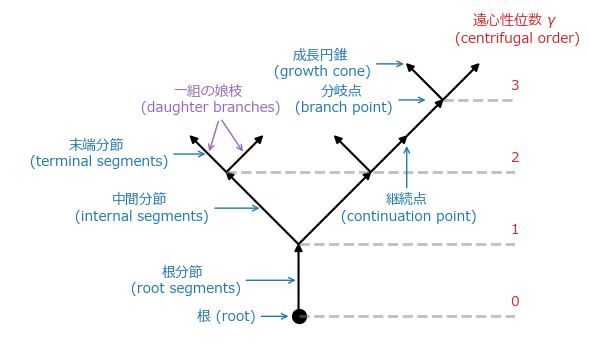
\includegraphics[scale=0.8, max width=\linewidth]{./fig/neuron-model/neurite-growth-model/cell009.png}
	\caption{cell009.png}
	\label{cell009.png}
\end{figure}
\subsection{様々な発火パターンのシミュレーション}
次に様々な発火パターンを模倣するようにIzモデルの定数を変化させてみよう.Intrinsically Bursting (IB)ニューロンとChattering (CH) ニューロン(または fast rhythmic bursting (FRB) ニューロン)のシミュレーションを行う.基本的には定数を変えるだけである.

本書で用いている式における発火パターンに対するパラメータは([Izhikevich, 2003](https://www.izhikevich.org/publications/spikes.htm))では得られないが,["Dynamical Systems in Neuroscience" (Izhikevich, 2007)](https://mitpress.mit.edu/books/dynamical-systems-neuroscience)には記載がある.他の発火パターンに関してはこの本を参照のこと.
\lstinputlisting[language=julia]{./text/neuron-model/izhikevich/011.jl}
これまでと異なり,モデルの定義時に\jl{param}を設定していることに注意しよう.最後に膜電位変化を描画する.
\lstinputlisting[language=julia]{./text/neuron-model/izhikevich/013.jl}
\begin{figure}[ht]
	\centering
	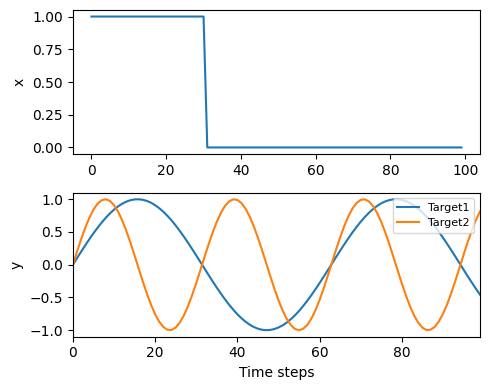
\includegraphics[scale=0.8, max width=\linewidth]{./fig/solve-credit-assignment-problem/bptt/cell013.png}
	\caption{cell013.png}
	\label{cell013.png}
\end{figure}
\subsection{ランダムネットワークのシミュレーション}
1000個のIzニューロン(興奮性800個, 抑制性200個)によるランダムネットワークのシミュレーションを行う.これは([Izhikevich, 2003](https://www.izhikevich.org/publications/spikes.htm))においてMATLABコードが示されており,それをJuliaに移植したものである.このシミュレーションではRS(regular spiking)ニューロンを興奮性細胞,FS(fast spiking)ニューロンを抑制性細胞のモデルとして用いている.
\lstinputlisting[language=julia]{./text/neuron-model/izhikevich/015.jl}
膜電位の更新の際,\jl{v}を2回に分けて更新しているが,これは数値的な安定性を高めるためである.計算量は上がるが,前述したモデルにおいても同様の処理を行う実装もある.

シミュレーションの実行後,ネットワークを構成するニューロンの発火を描画する.これを\textbf{ラスタープロット}\index{らすたーぷろっと@ラスタープロット} (raster plot)という.この図は横軸が時間,縦軸がニューロンの番号となっており,各ニューロンが発火したことを点で表している.
\lstinputlisting[language=julia]{./text/neuron-model/izhikevich/017.jl}
\begin{figure}[ht]
	\centering
	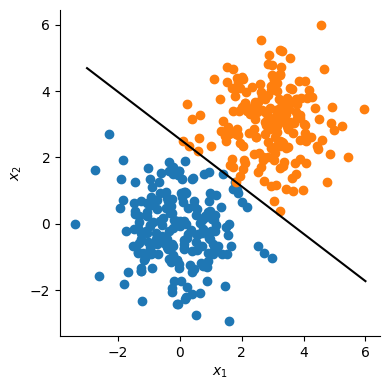
\includegraphics[scale=0.8, max width=\linewidth]{./fig/local-learning-rule/logistic-regression-perceptron/cell017.png}
	\caption{cell017.png}
	\label{cell017.png}
\end{figure}
初めの400msぐらいまでは100msごとに約10Hzの$\alpha$波が見られ,800ms付近には約40Hzの$\gamma$波が見られる.
